\documentclass[12pt,a4paper]{report}
\usepackage[utf8]{inputenc}
\usepackage{graphicx}
\usepackage{float}
\usepackage{hyperref}
\usepackage{xcolor}
\usepackage{setspace}
\usepackage{tabularx}

\hypersetup{
    colorlinks=true,
    linkcolor=black,
    filecolor=magenta,      
    urlcolor=cyan,
    pdftitle={Overleaf Example},
    pdfpagemode=FullScreen,
}

\onehalfspacing

\title{Chat Application Project Report}

\author{
  Project Group 6 -- DAT055
  \\ Hussein Hafid \\ Jan Rahimi \\ Mohamad Alzein \\ Zakaria Abulkadir
}
\date{\today}

\begin{document}
\maketitle

\begin{abstract}
  % Abstract of the report
  This report presents a chat application developed as part of the Object
  Oriented Applications (DAT055) course, featuring real-time text and image
  messaging alongside persistent data storage. The project adopts a client-server
  architecture, with a Java-based server managing user accounts, chat rooms, and
  database interactions via PostgreSQL, and a JavaFX client handling user
  interface and real-time updates. Core functionalities include account creation,
  login authentication, searching and joining chat rooms, and sending both text
  and images. Concurrency is achieved on the server side by dedicating a threaded
  handler to each incoming connection, while the client employs asynchronous
  listeners to avoid blocking graphical updates. The Model-View-Controller (MVC)
  pattern underpins the organization of client logic, enabling clear separation
  of concerns between scene rendering and network communication. Key challenges
  included establishing a robust TCP protocol, integrating multithreading with
  JavaFX, and coordinating team efforts with version control. Despite limitations
  in input validation and security, the resulting software fulfills essential
  requirements and serves as a foundation for potential enhancements such as
  encryption, refined UI features, and private chat rooms. This project
  highlights the importance of methodical design, careful concurrency management,
  and iterative development in creating a functional, scalable application.
\end{abstract}

\tableofcontents
\newpage

\chapter{Introduction}
% Introduction to the project and its objectives
This report documents the development of a chat application undertaken by a
team of students over an eight-week period. The chat application was created as
part of the Object Oriented Applications (DAT055) course and includes core
features such as user account creation, global chat rooms, real-time messaging
for text and images, and persistent data storage. The purpose of the project
was to gain practical experience with object-oriented design, concurrency,
JavaFX for graphical user interfaces, and relational database systems (in this
case, PostgreSQL). Throughout the process, emphasis was placed on applying
robust software engineering principles, including structured design patterns
and clear separation of concerns between client and server components.

\chapter{Project Requirements}
% Outline of the project requirements
The DAT055 course outlined a set of high-level requirements for the project.
The application was expected to handle multiple concurrent users who could
browse and connect to chat rooms, exchange messages reliably, and maintain a
persistent record of all conversations. The course specification also required
following a Model-View-Controller (MVC) pattern, ensuring that user
interaction, data manipulation, and presentation logic remained well-organized.
In particular, the final product needed a functioning graphical interface, as
well as support for both text and image messages within each chat.

% Interpretation of requirements
During early analysis, these requirements were interpreted to include the
creation of user accounts, joining multiple global chat rooms, sending and
receiving real-time messages, and storing all chat data in a format that
allowed users to retrieve previous conversation history. Additionally, the
course recommended the use of Java (including JavaFX or Swing) for the user
interface, along with guidance to properly cite any resources or AI tools
consulted during development.

\chapter{Scope of the Application}
% Scope and limitations of the application
This chat application is designed to address the central requirements, while
some functionalities remain deferred for future enhancements. The project
delivers a practical and direct chat system in which users can sign up or log
in, create or join chat rooms, and exchange text and image messages. The system
enforces minimal input validation, and users are permitted to choose any valid
username or email address, which are stored in the PostgreSQL database without
strict format checking. Although only a global chat environment exists in this
version, the structure allows potential expansion to private or invite-only
rooms later.

% Limitations and future enhancements
Since the project primarily serves as an educational exercise, it does not
implement certain advanced features that might be common in production systems,
such as strong password requirements, encryption for network traffic, or
sophisticated user role management. Despite these limitations, the basic
framework has been designed in such a way that these features could be added
later if time and resources permit.

% Initial design using CRC cards
\chapter{CRC Cards}

Before implementation, CRC (Class-Responsibility-Collaboration) cards were
created to outline the initial design of key classes. These cards helped
clarify class responsibilities and their interactions with other components of
the system. While the final implementation evolved beyond this initial
structure, the CRC approach provided valuable insights into defining the core
architecture of the chat application. The table bellow showcases the CRC cards
we designed in the early design phase of the project:

\begin{table}[H]
  \centering
  \renewcommand{\arraystretch}{1.4} % Increases row spacing for better readability
  \setlength{\tabcolsep}{8pt} % Adjusts column spacing to fit within margins
  \resizebox{0.92\textwidth}{!}{ % Resizes table to 92% of text width to avoid edge clipping
    \begin{tabular}{|p{4cm}|p{8cm}|p{4.5cm}|}
      \hline
      \textbf{Class Name}         & \textbf{Responsibilities}                                                                                                                            & \textbf{Collaborators}                                                           \\
      \hline
      \texttt{UserController}     & Manages user-related actions, such as login and logout. Communicates with the \texttt{AccountHandler} to retrieve user data and validate operations. & \texttt{AccountHandler}                                                          \\
      \hline
      \texttt{MessageController}  & Handles user interactions related to messages. Forwards requests to the \texttt{MessageHandler} and validates input.                                 & \texttt{MessageHandler}                                                          \\
      \hline
      \texttt{ChatroomController} & Manages chatroom-related interactions, including joining, leaving, and creating chat rooms. Relays data to the \texttt{ChatHandler}.                 & \texttt{ChatHandler}                                                             \\
      \hline
      \texttt{AccountHandler}     & Interfaces with the database to manage user authentication, account creation, and deletion. Ensures secure handling of user credentials.             & \texttt{Model}, \texttt{UserController}                                          \\
      \hline
      \texttt{MessageHandler}     & Manages message data, including storage, retrieval, and deletion. Interacts with the database to persist message history.                            & \texttt{Model}, \texttt{MessageController}                                       \\
      \hline
      \texttt{ChatHandler}        & Manages chatroom data, including creation, deletion, and membership tracking. Updates the model with chatroom state changes.                         & \texttt{Model}, \texttt{ChatroomController}                                      \\
      \hline
      \texttt{Model}              & Centralized data storage for users, messages, and chat rooms. Interfaces with the database to persist user activity.                                 & \texttt{MessageHandler}, \texttt{ChatHandler}, \texttt{AccountHandler}           \\
      \hline
      \texttt{View}               & Renders the user interface, including login screens, chat rooms, and message history. Relays user inputs to controllers.                             & \texttt{MessageController}, \texttt{UserController}, \texttt{ChatroomController} \\
      \hline
      \texttt{User}               & Represents user-related data, such as usernames and authentication status. Provides methods for retrieving or updating user attributes.              & \texttt{Model}, \texttt{AccountHandler}                                          \\
      \hline
      \texttt{Message}            & Represents an individual message, including sender, content, and timestamp. Provides methods for message creation and modification.                  & \texttt{Model}, \texttt{MessageHandler}                                          \\
      \hline
      \texttt{ChatRoom}           & Represents a chatroom, including its name, participants, and message history. Manages operations specific to chat rooms.                             & \texttt{Model}, \texttt{ChatHandler}                                             \\
      \hline
    \end{tabular}
  }
  \caption{CRC Cards for the Chat Application}
  \label{crc_cards}
\end{table}

\chapter{Design of the Chat Application}
\section{Overview}
The chat application follows a client-server architecture, where a dedicated
server manages all chat room data and user authentication while clients connect
to the server to interact with chat rooms. The application is designed using
Java, with PostgreSQL for data persistence and JavaFX for the graphical user
interface. The communication between the client and the server is facilitated
using TCP sockets, allowing real-time message exchange.

\section{Server-Side Design}
The server is responsible for handling multiple client connections, managing
chat rooms, storing messages, and processing user authentication. The main
component of the server is the \texttt{ChatServer}, which listens for incoming
TCP connections and assigns a dedicated \texttt{ClientHandler} to each
connected user. The server also includes a \texttt{NotificationHandler} that
listens for changes in the database and notifies relevant clients when new
messages arrive.

\begin{figure}[H]
  \centering
  % Replace "server_class_diagram.png" with your actual image file
  \includegraphics[width=0.9\textwidth]{Server.png}
  \caption{Server Application Class Diagram}
  \label{fig:server_class_diagram}
\end{figure}

\section{Client-Side Design}
The client application follows the Model-View-Controller (MVC) pattern,
ensuring a clear separation of concerns between data handling, user interface,
and server communication. The user interface is managed through JavaFX, where a
\texttt{SceneManager} dynamically loads different views, such as the login
screen, main chat view, and settings page. Communication with the server is
handled through \texttt{ClientSender} and \texttt{ClientReceiver}, which ensure
that messages and commands are sent and received asynchronously.

\begin{figure}[H]
  \centering
  % Replace "client_class_diagram.png" with your actual image file
  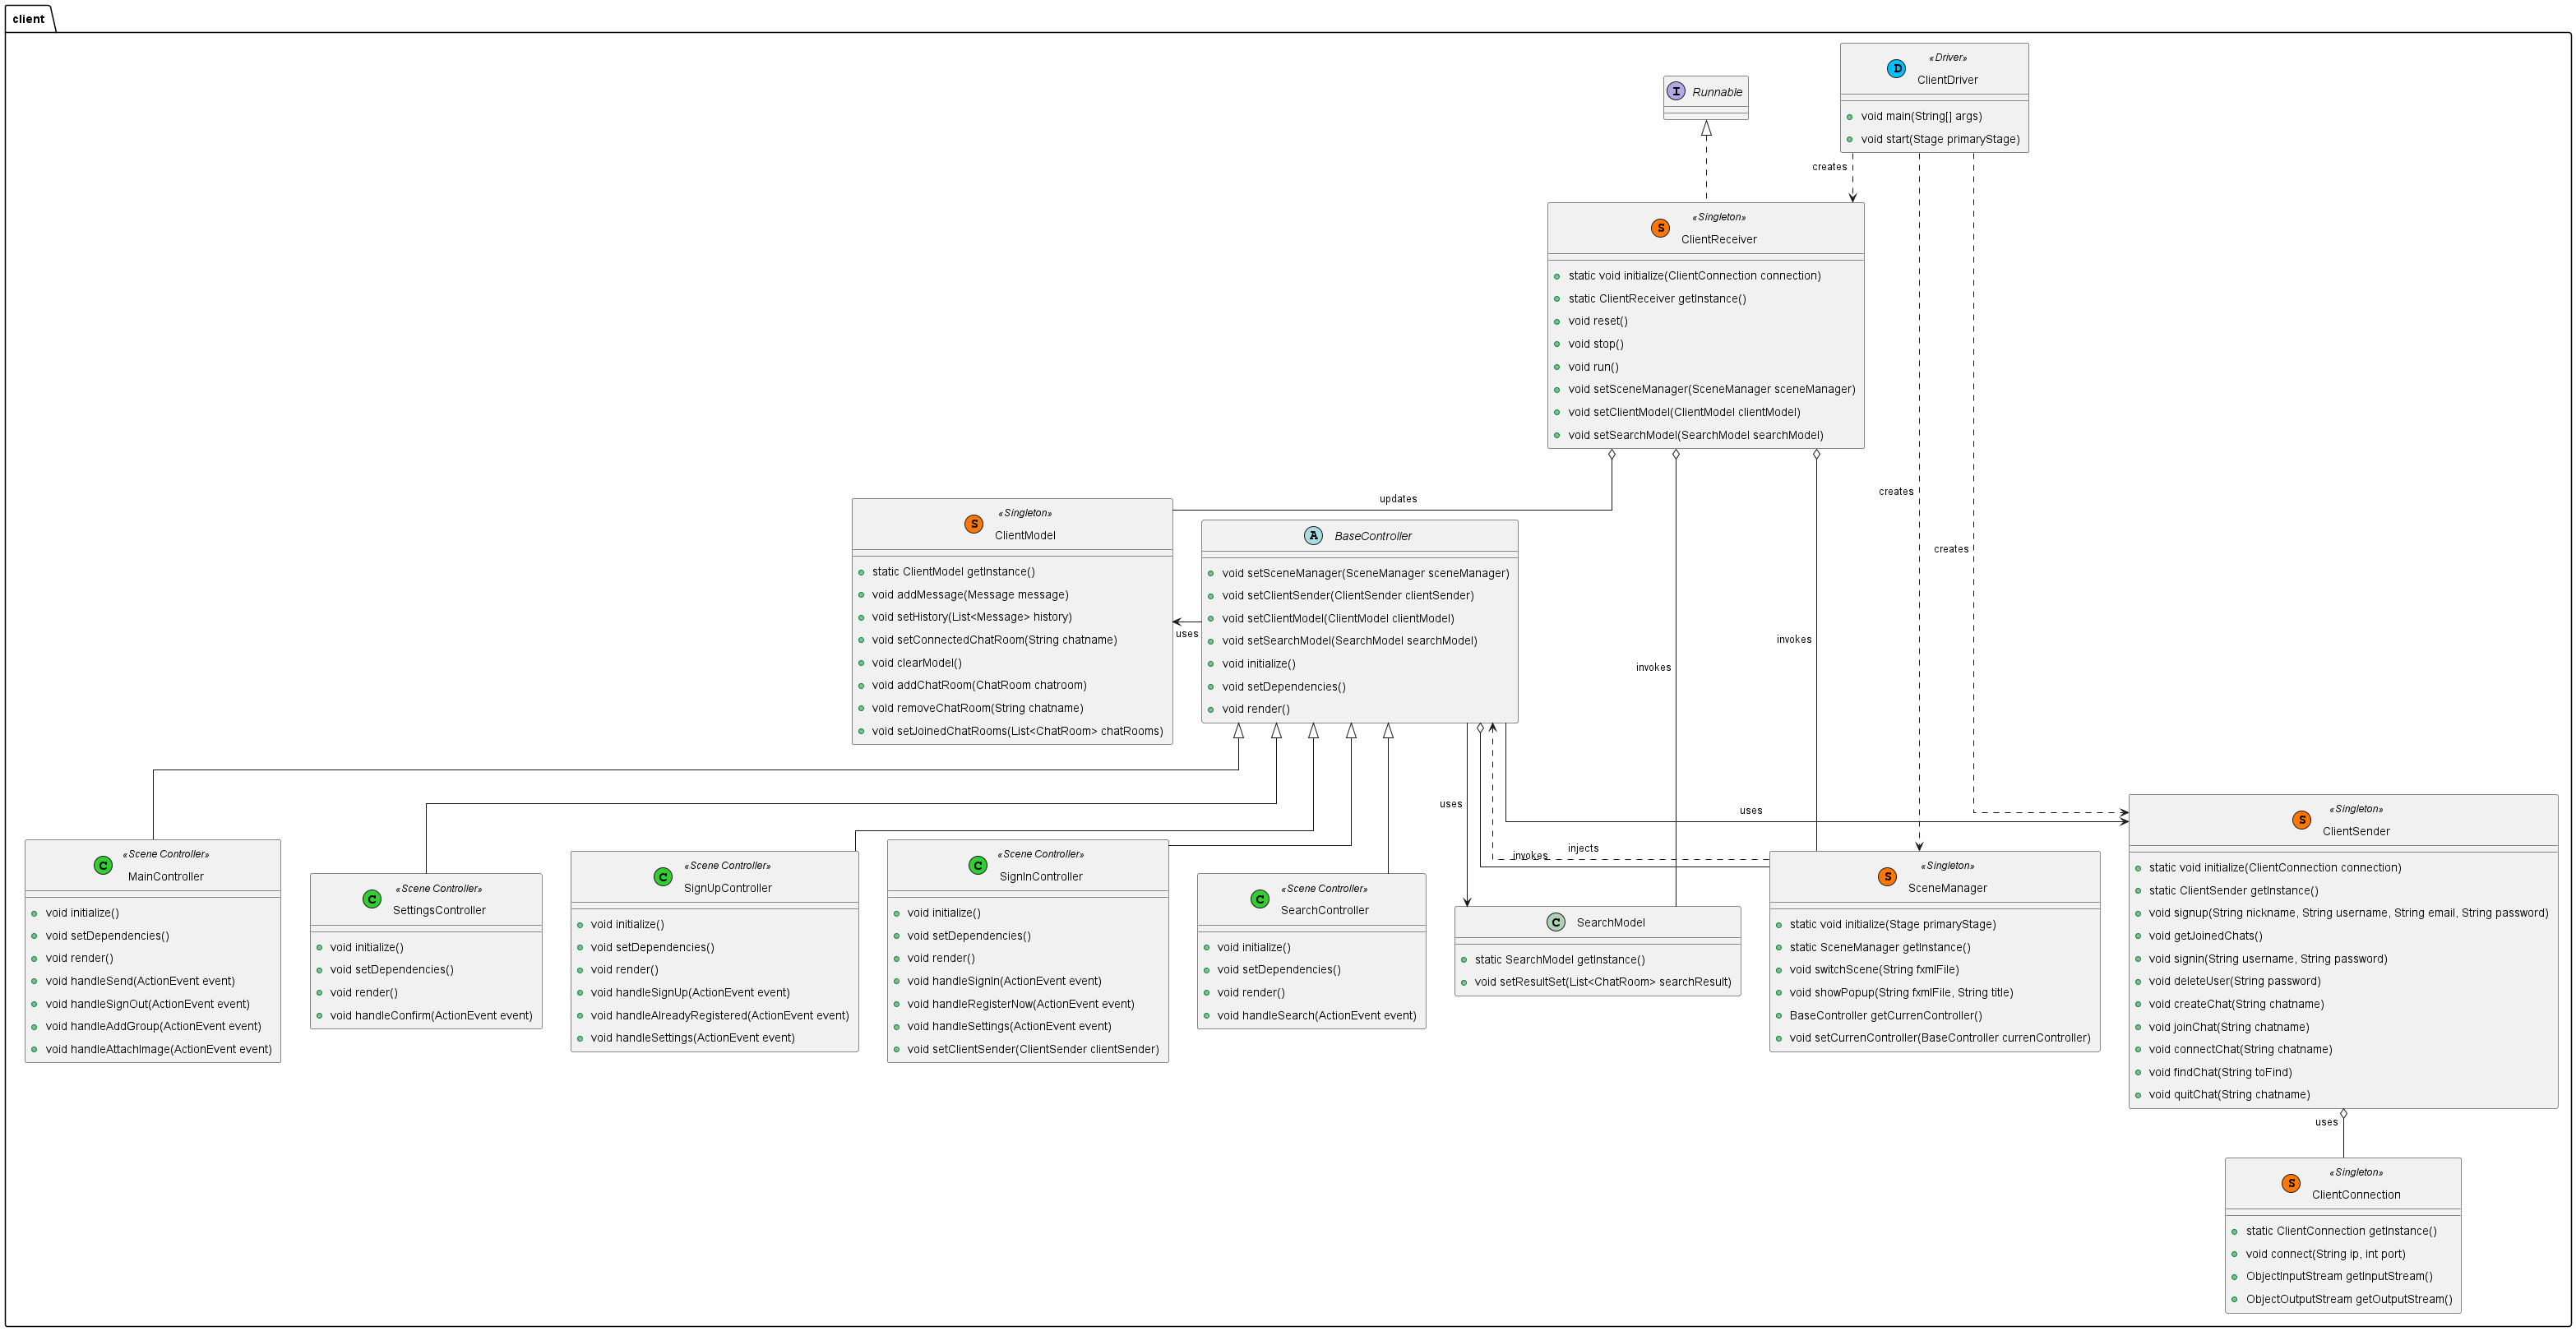
\includegraphics[width=0.9\textwidth]{client.png}
  \caption{Client Application Class Diagram}
  \label{fig:client_class_diagram}
\end{figure}

\section{Client State Diagram}
The client transitions between multiple states throughout its lifecycle.
Initially, the client is in a \textit{Disconnected} state. Once a connection is
established with the server, the client moves into the \textit{Connected}
state. After successful authentication, the client enters the
\textit{Authenticated} state. The client remains in this state until it joins a
chat room, at which point it transitions to the \textit{Connected to Chat Room}
state. If the connection is lost, the client returns to the
\textit{Disconnected} state.

\begin{figure}[H]
  \centering
  % Replace "client_state_diagram.png" with your actual image file
  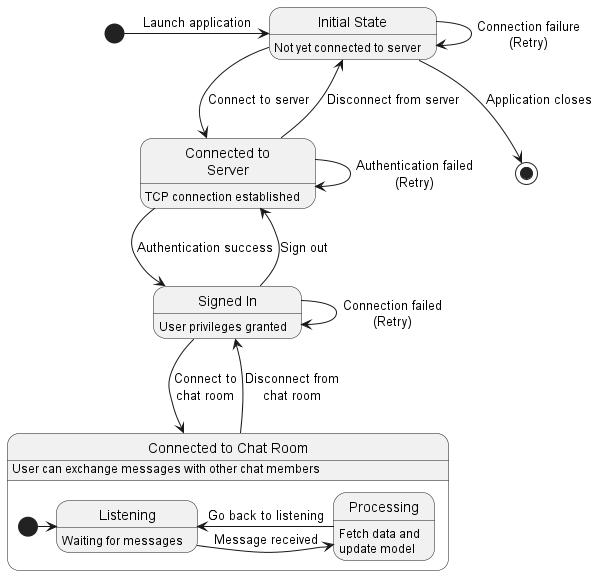
\includegraphics[width=0.9\textwidth]{state.png}
  \caption{Client State Diagram}
  \label{fig:client_state_diagram}
\end{figure}

\section{Login Procedure Sequence Diagram}
The login procedure consists of several interactions between the client and the
server. When a user enters their credentials and submits the login request, the
client sends a \texttt{signin} command to the server. The server then verifies
the credentials by querying the database. If the login is successful, the
server responds with a success message, and the client transitions to the main
chat view.

\begin{figure}[H]
  \centering
  % Replace "login_sequence_diagram.png" with your actual image file
  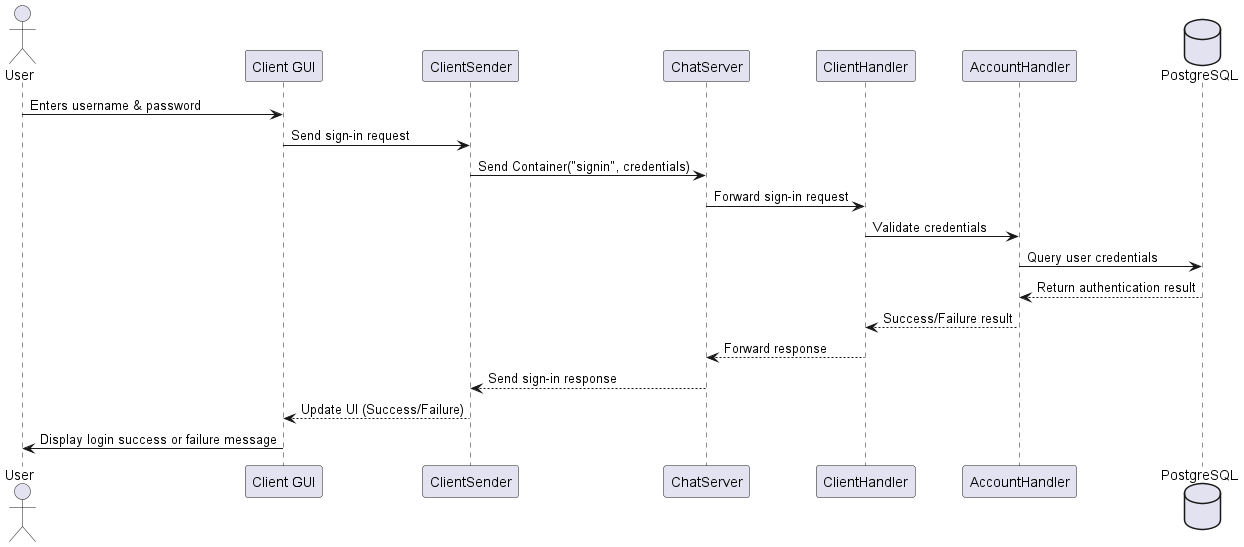
\includegraphics[width=0.9\textwidth]{signin.png}
  \caption{Login Procedure Sequence Diagram}
  \label{fig:login_sequence_diagram}
\end{figure}

\chapter{Implementation and Design Improvements}
% Improvements made during implementation
The design underwent several improvements during implementation. One of the
foremost decisions was to adopt a relational database for storing all
persistent data, including user credentials, chat rooms, and messages. This
choice simplified data access patterns and improved reliability. Another key
improvement emerged in the approach to concurrency: the team decided to run
each connected client on its own thread in the server, making it feasible to
handle multiple simultaneous chat operations without one client blocking
another.

% Use of Container objects
Additionally, the introduction of \texttt{Container} objects to package
commands and arbitrary data proved efficient. Even though this strategy carries
risks (such as sending large or maliciously crafted objects), it served as a
quick solution to achieve a functioning protocol. Future iterations might adopt
a more secure approach, such as sending JSON messages over encrypted channels,
to better protect sensitive data.

\chapter{Workflow}
% Description of the workflow and team collaboration
Early in the project, a Waterfall-like approach was planned, with defined
phases for requirements, design, and implementation. In practice, the team
found that changes to the design were often necessary while coding was
underway, leading to partial overlap of tasks. The attempt to split the team
into server-side and client-side subgroups was only partially successful, as
some members had limited availability or experience. The resulting imbalance
meant that major architectural decisions were occasionally made by a smaller
subset of the team.

% Version control challenges and improvements
Version control with Git and GitHub initially posed difficulties, especially
with merging branches and preventing conflicts. It was discovered that working
directly on the \texttt{main} branch caused significant confusion. Only in the
later stages was a more systematic approach adopted, allowing pull requests to
be used for code reviews and merges. This shift improved code quality and
reduced the likelihood of major regressions.

\chapter{Running the Application}
\section{Server Application}
% Instructions for running the server application
The server can be compiled using Maven or by invoking a \texttt{make} command
if the provided automation scripts are used. After configuring PostgreSQL
through the project's initialization steps, running the \texttt{ServerDriver}
class starts the application in listening mode. The server remains active,
awaiting incoming TCP connections on the specified port. Notifications from the
database are listened to in a dedicated thread, so any insertion of new
messages triggers updates to the subscribed clients.

\section{Client Application}
% Instructions for running the client application
The client requires JavaFX libraries and can similarly be launched by compiling
and running the \texttt{ClientDriver} class. Upon startup, the client presents
a Sign-In View, but it is first necessary to configure the server's IP address
and port within the Settings View. Once the socket connection is established,
the user can log in or register for an account. Successful login transitions to
the Main View, which displays joined chat rooms, allows searching or creating
new rooms, and provides a means to send text or image messages in real time.

\chapter{System Requirements}
% System requirements for running the application
The application relies on Java 22 or higher, as well as a Bash shell and
\texttt{make} for automating the setup process. On the server side, PostgreSQL
must be installed and running, typically at version 15 or higher, with proper
network accessibility for the client. The client side requires JavaFX, although
Maven is used to pull in dependencies automatically. Firewall or network
restrictions may impede successful connections, as the system expects an open
TCP port on the server host.

\chapter{Usage}
% Usage instructions for the application
When starting the client, the Sign-In View appears. If an account already
exists, the user can provide a username and password to authenticate.
Otherwise, a link in the Sign-In View navigates to the Sign-Up View, where new
credentials may be registered. Once logged in, the Main View appears and
displays all joined chat rooms on the left, with a chat container in the center
for messages. A text field permits entering and sending text, while an “Attach
Image” button opens a file chooser to send images in PNG, JPG, or GIF formats.

% Additional usage details
The Main View also features an “Add” button that opens the Search View. In that
scene, users can search for existing chat rooms by name or create a new one.
Upon locating a desired room, selecting it automatically issues a join request
to the server; a successful join results in that room appearing in the Main
View’s list. By clicking on a joined room, the system retrieves the message
history from the server and listens for new incoming messages. This mechanism
relies on the notification functionality implemented server-side, which
broadcasts changes to all connected members in real time.

\chapter{Use of AI in the Project}
\label{ch:ai_usage}

Artificial Intelligence (AI) tools were leveraged throughout the development of
this project to enhance productivity, facilitate problem-solving, and improve
the quality of both the implementation and documentation. The use of AI was
guided by ethical considerations, ensuring that AI-assisted content was
reviewed, refined, and integrated responsibly.

AI played a significant role in assisting with software development,
particularly in debugging and optimizing code. During the implementation phase,
AI tools were consulted for identifying and resolving syntax errors, runtime
exceptions, and logic flaws. Additionally, AI provided suggestions for
optimizing Java concurrency, socket communication, and database interactions.
It also offered guidance on best practices for structuring the client-server
architecture and assisted in configuring PostgreSQL, Maven dependencies, and
JavaFX. Despite AI's assistance in debugging, all final decisions regarding
code modifications were made manually, ensuring that AI-generated suggestions
aligned with the intended functionality and course requirements.

Throughout the project, AI tools were used as a research assistant to
efficiently find relevant documentation, tutorials, and technical references.
This included locating official Java and PostgreSQL documentation,
understanding JavaFX scene management and event handling, gathering information
on best practices for using TCP sockets in Java, and exploring design patterns,
including the Model-View-Controller (MVC) architecture. While AI provided
guidance in locating useful resources, all external references were verified
for accuracy before being implemented.

Given the complexity of structuring a formal project report, AI was employed to
assist in formatting and organizing the document. It played a key role in
structuring the report according to standard academic formatting, ensuring
proper LaTeX styling for tables, figures, citations, and complex document
elements. AI was particularly valuable in generating LaTeX-compatible UML
diagrams and sequence diagrams, enhancing readability and coherence by refining
explanations and transitions between sections. By leveraging AI's proficiency
in LaTeX, the report benefited from well-formatted CRC card tables, structured
sequence diagrams, and neatly aligned code snippets.

All AI-assisted content was critically reviewed and refined before inclusion in
the final submission. AI was not used for direct code generation but rather as
an advisory tool to streamline development, improve efficiency, and enhance
documentation. The final report reflects the project team's understanding and
manual adjustments to AI-assisted outputs, ensuring originality and academic
integrity. The integration of AI tools into the project workflow significantly
improved efficiency in debugging, research, report structuring, and LaTeX
formatting. However, AI was used strictly as a consultative tool rather than as
a replacement for critical thinking, problem-solving, or implementation. The
final product represents the collective efforts of the team, with AI serving as
a supplementary resource for enhancing productivity and documentation quality.

\chapter{Discussion}
% Discussion of the development process and challenges
Development proceeded with sporadic adherence to the Waterfall methodology.
Early design documents, such as CRC cards, did not entirely capture the
eventual client-server separation that was decided upon. Challenges included
dealing with Java sockets and concurrency, establishing database connections
through a connection pool, and integrating JavaFX while maintaining responsive
performance. Some team members encountered scheduling or experience barriers,
creating an uneven distribution of workload. As a result, the project’s
leadership role became more concentrated among a few contributors who managed
both conceptual design and a significant portion of the coding.

% Major difficulties and security concerns
The major difficulties ranged from merging Git branches without causing code
conflicts, to ensuring correct synchronization among threads that handled
network input, broadcast notifications, and the JavaFX UI. In addition, storing
passwords in plaintext, and transmitting them unencrypted, stands out as a
security risk. While the project scope did not prioritize advanced security
measures, future improvements would address these concerns. Nevertheless, the
completed application meets essential requirements, and the experience provided
insights into concurrency, database design, and user interface implementation.

\chapter{Conclusion}
% Conclusion summarizing the project outcomes
The chat application project demonstrates how a client-server system can be
built in Java, employing both concurrency and a GUI framework. Despite
challenges that arose from limited collaboration among team members, the final
solution supports real-time text and image messaging, user authentication, and
persistent data storage with PostgreSQL. The project’s evolution reveals the
importance of flexible design, thorough testing, and effective communication
within a team. Although certain limitations remain—particularly around security
and feature depth—the application serves as a functional foundation that could
be extended or refined in future iterations.

\chapter{Future Improvements and Enhancements}
% Future improvements and enhancements
While the basic requirements are fulfilled, several significant enhancements
are anticipated. One key priority involves improving security, such as adding
encryption for client-server communications and adopting password hashing and
salting. Another improvement would be validating user input more rigorously,
especially for email addresses, usernames, and passwords. Introducing advanced
chat features, including private or invite-only rooms, message replies, or an
advanced user roles system, could further enrich the user experience. Better
packaging for distribution, such as generating .jar files or Docker images, may
also prove useful in making the application accessible to a broader audience
without requiring in-depth knowledge of Maven or Git.

% \chapter{Sample Code}
% % Sample code snippet from the project
% A crucial part of the project involves handling client requests on the server
% side. The following snippet from \texttt{ClientHandler.java} illustrates how
% the server processes different commands by examining the \texttt{command} field
% within a \texttt{Container} object:

% \bigskip
% \noindent
% \begin{verbatim}
% private Container executeCommand(Container container) {
%     String command = container.getCommand();
%     Object data = container.getData();
%     switch (command) {
%         case "signin":
%             return handleSignin(data);
%         case "signup":
%             return handleSignup(data);
%         ...
%         default:
%             return new Container("error", "Unknown command: " + command);
%     }
% }
% \end{verbatim}

% Additional sample code
Additional sample code, such as the \texttt{ClientReceiver} that runs on the
client side to handle background communication, provides a complementary view
of how messages flow from the server to the user interface in real time.

\appendix
\chapter{Additional Resources}
% Additional resources and references
\section*{Repository}
You can visit our repository at: \\
\hyperlink{https://github.com/Zakoroo/Project-Group-6}{https://github.com/Zakoroo/Project-Group-6}

\end{document}
